\documentclass[]{report}
% Title Page
\usepackage[utf8]{inputenc}
\usepackage[T1]{fontenc}
\usepackage[polish]{babel}
\usepackage{graphicx}
\usepackage{listings}
\usepackage{listings}
\usepackage{geometry}
\usepackage{xcolor}
\usepackage{subcaption}
\usepackage{hyperref}
\usepackage{float}
\usepackage{placeins}
\geometry{a4paper, left=2cm, right=2cm, top=2cm, bottom=2cm}
\lstset{
	language=C++,
	basicstyle=\ttfamily,
	keywordstyle=\color{blue},
	commentstyle=\color{green!40!black},
	stringstyle=\color{red},
	numbers=left,
	numberstyle=\tiny,
	stepnumber=1,
	numbersep=5pt,
	backgroundcolor=\color{white},
	frame=single,
	breaklines=true,
	breakatwhitespace=true,
	tabsize=4,
	captionpos=b,
	caption=\lstname,
	extendedchars=true,
	inputencoding=utf8,
	literate={ą}{{\k{a}}}1 {ć}{{\'c}}1 {ę}{{\k{e}}}1 {ł}{{\l{}}}1 {Ł}{{\L{}}}1 {ń}{{\'n}}1 {ó}{{\'o}}1 {ś}{{\'s}}1 {Ś}{{\'S}}1  {ź}{{\'z}}1 {ż}{{\.z}}1,}

\begin{document}

	
\begin{titlepage}
	\centering

	\vspace{1cm}
	
	
\includegraphics[width=1.0\textwidth]{logowmit.png} % Mniejsze zdjęcie
	
	\vspace{1cm}
	
	Kierunek: Inżynieria i Analiza Danych % Tekst "Kierunek"
	
	\vspace{1.5cm}
	
\includegraphics[width=0.3\textwidth]{PL.jpeg} % Mniejsze zdjęcie
	
	\vspace{1cm}
	{\scshape\Large Wisielec \par} % Temat raportu
	
	\vspace{1.5cm}
	{\Large Bartosz Oleszek, Katarzyna Zyśko, Zuzanna Winiarska \par} % Autorzy
	
	\vfill
	{\large \today\par}
\end{titlepage}


\tableofcontents
	
\newpage 


	\section*{Wprowadzenie}
	\addcontentsline{toc}{section}{1. Wstęp}
	
	Wisielec to interaktywna gra słowno-logiczna, w której gracze testują swoją zdolność do odgadywania słów poprzez wprowadzanie pojedynczych liter. Gra została stworzona w języku C++ przy użyciu biblioteki wxWidgets, umożliwiającej dynamiczny interfejs graficzny. Inspiracją do tego projektu był klasyczny hangman (wisielec) dostępny na wielu platformach.
	
	\subsection*{Cel projektu}
	\addcontentsline{toc}{subsection}{1.1 Cel projektu}
	
Gra "Wisielec" to interaktywna aplikacja napisana w języku C++, wykorzystująca bibliotekę wxWidgets. Celem projektu jest dostarczenie użytkownikowi przyjemnej rozrywki, jednocześnie rozwijając umiejętności logicznego myślenia oraz słownikowe. Gra opiera się na odgadywaniu słów, co pozwala ćwiczyć zdolności związane z spostrzegawczością, dedukcją i umiejętnością radzenia sobie w sytuacjach, w których konieczne jest podejmowanie decyzji na podstawie ograniczonych informacji.
	
	\subsection*{Cel Gry}
	\addcontentsline{toc}{subsection}{1.1 Cel gry}
	
Celem gry "Wisielec" jest dostarczenie rozrywki i jednocześnie rozwijanie umiejętności logicznego myślenia poprzez odgadywanie ukrytych słów. Gracz stawia sobie za zadanie odgadnąć słowo przed przekroczeniem limitu błędnych prób. Punkty są przyznawane za poprawne odgadnięcia, a statystyki gracza motywują do poprawy wyników. Gra łączy zabawę z edukacją, rozwijając spostrzegawczość i dedukcję.
	
	\subsection*{Zasady Gry}
	\addcontentsline{toc}{subsection}{1.2 Zasady gry}
	
	\begin{itemize}
		\item Gra prezentuje graczowi ukryte słowo za pomocą pustych miejsc reprezentowanych podkreśleniem "\_". Gracz musi odgadnąć literę, wprowadzając ją do pola tekstowego.
		\item Po wprowadzeniu litery, program sprawdza, czy litera znajduje się w słowie. Jeśli tak, odkrywa odpowiednie miejsce w słowie, a gracz kontynuuje odgadywanie.
		\item Jeśli litera nie występuje w słowie, program rysuje element wisielca. Gracz ma ograniczoną liczbę prób, zanim zostanie ukazany cały wisielec, co oznacza przegraną.
		\item Gracz ma także możliwość skorzystania z przycisku podpowiedzi, który wyświetli jedną literę w słowie, jednak za cenę utraty punktów.
		\item Po zdobyciu 5 zwycięstw, gracz otrzymuje wirtualny brązowy puchar, co stanowi wyróżnienie za osiągnięcia w grze. Kolejne wyróżnienie, srebrny puchar, przyznawane jest po uzyskaniu 10 zwycięstw. Dla najbardziej wytrwałych graczy, po 15 zwycięstwach przewidziany jest złoty puchar, symbolizujący najwyższy poziom umiejętności w odgadywaniu słów. 
		
		
	\end{itemize}
\newpage
\section*{Elementy Interfejsu Graficznego}
\addcontentsline{toc}{section}{2. Elementy Interfejsu graficznego}

Interfejs graiczny gry \textit{"Wisielec"} (rysunek~\ref{fig:Interfejs}) został starannie zaprojektowany, aby zapewnić użytkownikowi intuicyjne i przyjemne doświadczenie podczas zgadywania słów. Składa się z kilku kluczowych elementów, które nie tylko ułatwiają rozgrywkę, ale także dostarczają istotnych informacji o stanie gry.

\subsection*{1. Okno główne}
\addcontentsline{toc}{subsection}{2.1 Okno główne}

Okno główne to główny obszar interakcji w grze $"Wisielec"$, gdzie odbywa się cała rozgrywka i umieszczone są wszystkie elementy interfejsu użytkownika. Dodatkowo, gracz może zminimalizować lub zamknąć okno za pomocą przycisków systemowych w prawym górnym rogu, co umożliwia mu chwilowe ukrycie gry lub zakończenie rozgrywki.

\subsection*{2. Pole zgadywanego słowa}
\addcontentsline{toc}{subsection}{2.2 Pole zgadywanego słowa}

W górnej części okna wyświetlane jest pole do zgadywania słowa, z serią pustych pól (w formie ciągu $"\_"$) zastąpionych literami po każdej poprawnej odpowiedzi gracza. To miejsce jest centralnym punktem interakcji, gdzie gracz monitoruje postępy w odgadywaniu słowa. Dodatkowo, można tu otrzymać podpowiedzi po naciśnięciu odpowiedniego przycisku.

\subsection*{3. Kategoria}
\addcontentsline{toc}{subsection}{2.3 Kategoria}

Poniżej pola zgadywanego słowa znajdują się informacje o kategorii, do której należy słowo, oraz liczba zdobytych punktów przez gracza. Kategoria dostarcza dodatkowego kontekstu dotyczącego słowa, co może pomóc graczowi w dedukowaniu jego zawartości.

\subsection*{4. Liczba punktów}
\addcontentsline{toc}{subsection}{2.4 Lliczba punktów}

Liczba punktów, oznaczonych w interfejsie jako błękitne diamenty, motywuje graczy do poprawnego zgadywania słów i stanowi walutę, którą mogą wymieniać na podpowiedzi ułatwiające rozgrywkę. Jej wyświetlanie pozwala graczom śledzić swój postęp i podejmować decyzje dotyczące dalszej rozgrywki.

\subsection*{5. Obszar rysowania postaci wisielca}
\addcontentsline{toc}{subsection}{2.5 Obszar rysowania postaci wisielca}

Pod informacjami o słowie, kategorii i liczbie punktów znajduje się obszar, gdzie rysowana jest postać wisielca. Stopniowo, w miarę postępu rozgrywki i popełniania błędów przez gracza, dodawane są kolejne elementy postaci, co tworzy wizualną reprezentację stanu gry. Gracz może obserwować rozwój postaci, co dodaje emocji i dynamiki do rozgrywki.

\subsection*{6. Przycisk podpowiedzi}
\addcontentsline{toc}{subsection}{2.6 Przycisk podpowiedzi}

Przycisk podpowiedź, wyświetlany w formie grafiki żarówki, znajduje się obok obszaru rysowania postaci wisielca. Kliknięcie tego przycisku wyświetla dodatkową wskazówkę, która może pomóc graczowi w odgadnięciu słowa. Nad przyciskiem wyświetlana jest również informacja o cenie podpowiedzi, co informuje gracza o koszcie skorzystania z tej opcji.

\subsection*{7. Pole do wpisywania odpowiedzi}
\addcontentsline{toc}{subsection}{2.7 Pole do wpisywania podpowiedzi}

W centralnej części interfejsu znajduje się pole tekstowe, które służy do wprowadzania odpowiedzi. To pole stanowi główne narzędzie interakcji, gdzie gracz aktywnie uczestniczy w rozgrywce, podejmując decyzje i wprowadzając litery w celu zgadywania słowa. Jest to kluczowy element interfejsu, który umożliwia graczowi bezpośrednie zaangażowanie się w rozgrywkę i prowadzenie procesu odgadywania.

\subsection*{8. Lista użytych liter}
\addcontentsline{toc}{subsection}{2.8 Lista użytych liter}

Pod polem do wpisywania odpowiedzi znajduje się obszar, w którym wyświetlana jest lista liter, które zostały już użyte w trakcie rozgrywki. To pomaga uniknąć powtórek i śledzić postępy.

\subsection*{9. Wyświetlanie pucharu i liczby zwycięstw}
\addcontentsline{toc}{subsection}{2.9 Wyświetlanie pucharu i liczby zwycięstw}

W dolnej części okna znajduje się obszar, w którym prezentowane są informacje o pucharze (gdy liczba zwycięstw $\geq5$) oraz liczbie wygranych. Kolor pucharu może się zmieniać w zależności od liczby zwycięstw gracza, co dodaje elementu motywującego do dalszej gry.

\subsection*{10. Przycisk "nowe słowo"}
\addcontentsline{toc}{subsection}{2.10 Przycisk $"$nowe słowo$"$}

Na samym dole okna znajduje się przycisk $"$nowe słowo$"$, który pozwala na rozpoczęcie nowej rundy. Po jego kliknięciu losowane jest nowe słowo do odgadnięcia, umożliwiając graczowi kontynuację rozgrywki.
\\

\begin{figure}[h]
	\centering
	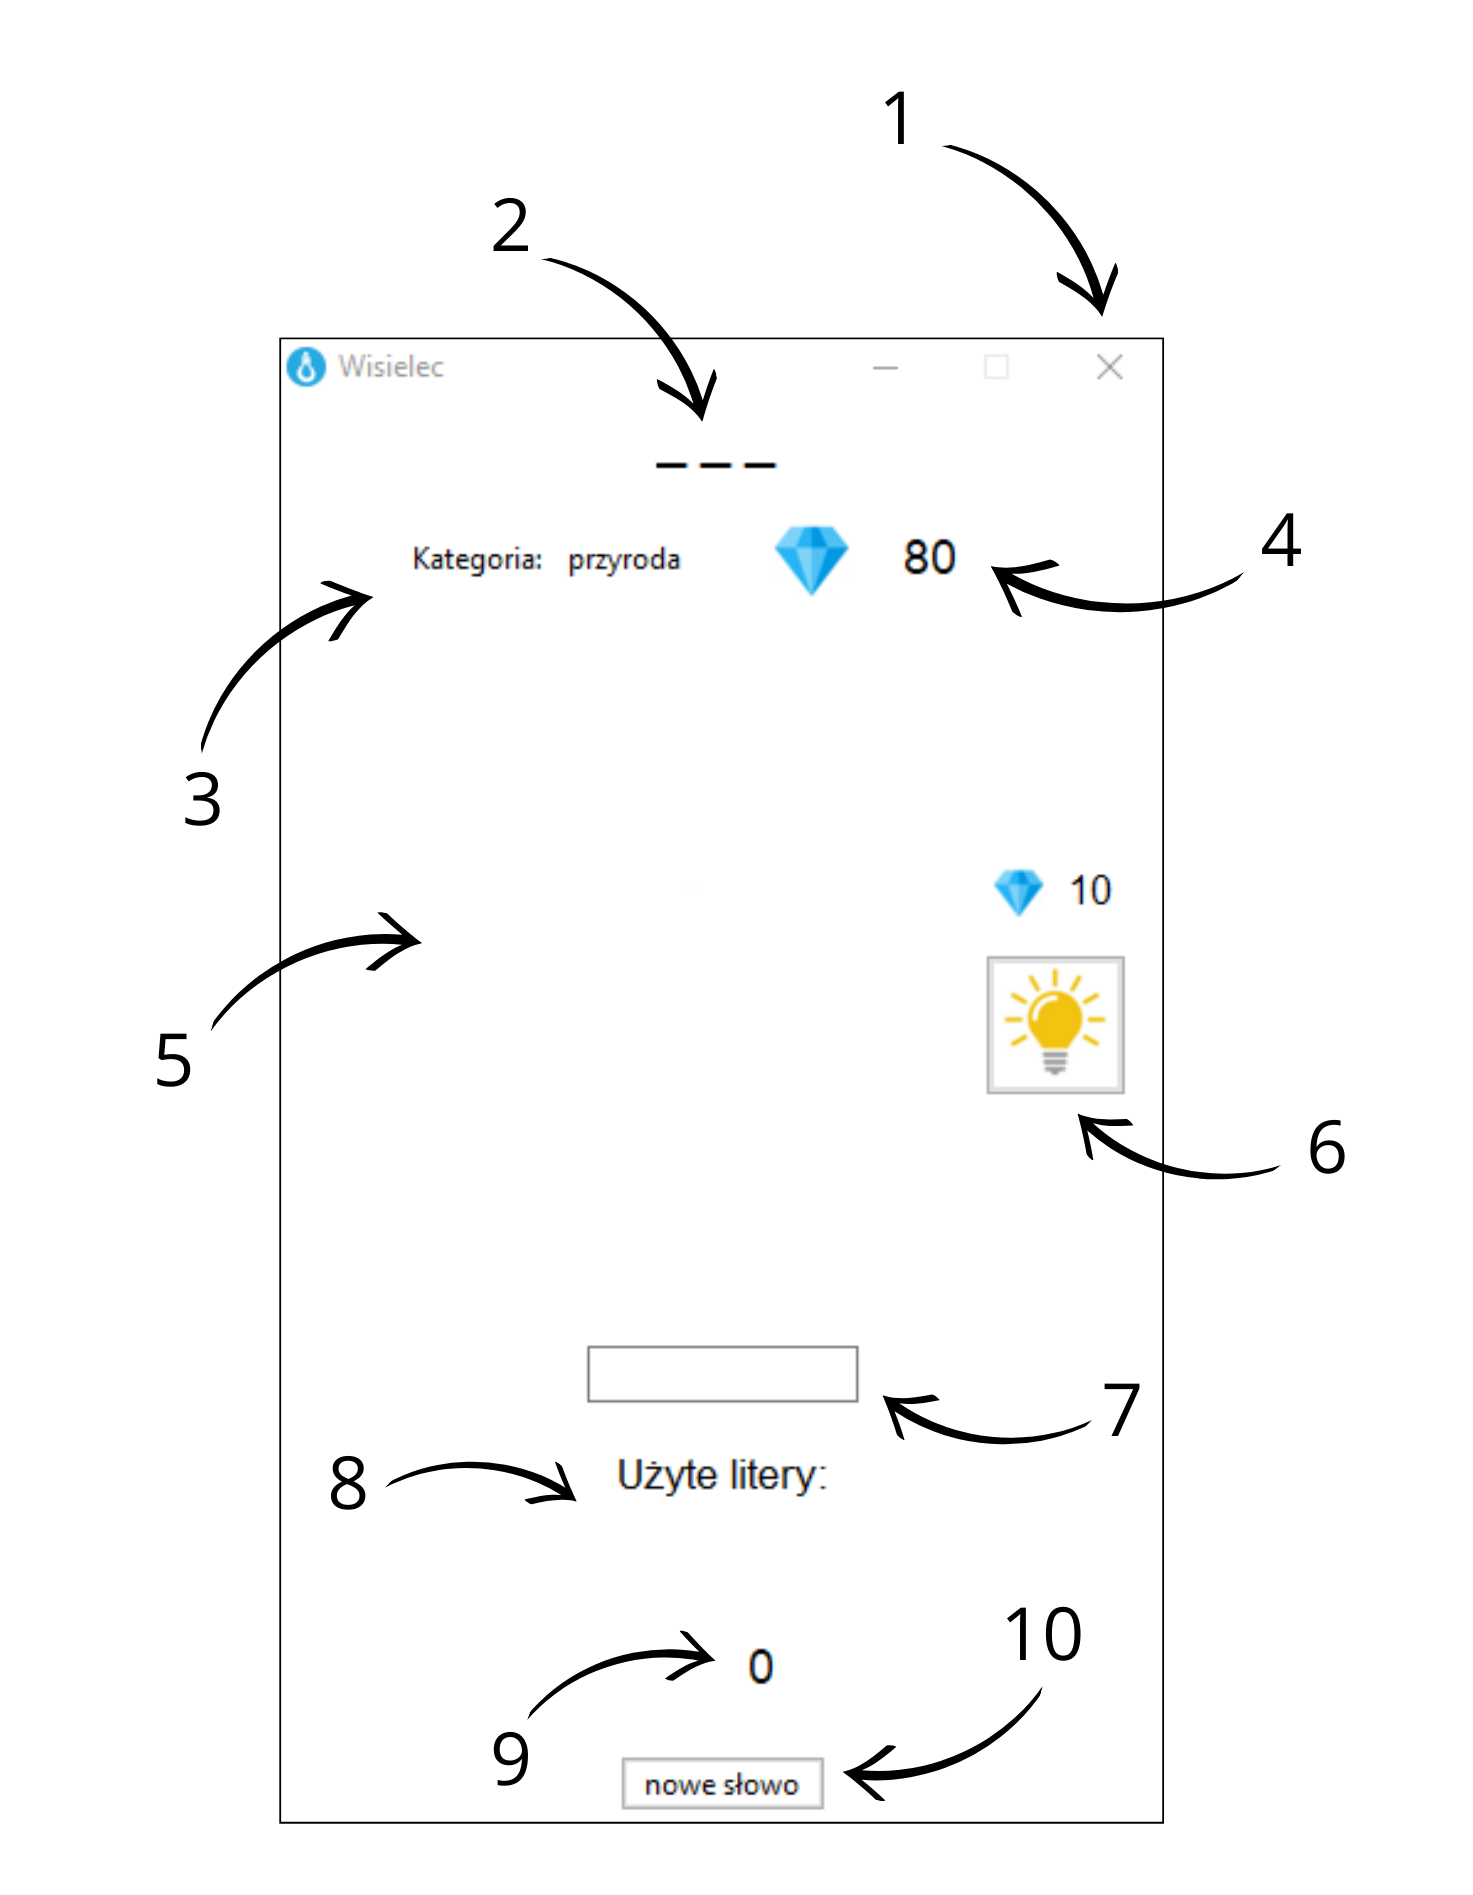
\includegraphics[width=0.7\textwidth]{interface}
	\caption{Interfejs gry}
	\label{fig:Interfejs}
\end{figure}

\newpage
\section *{Rozgrywka}
\addcontentsline{toc}{section}{3. Rozgrywka}

Rozgrywka gry $"Wisielec"$ polega na odgadywaniu słowa poprzez wprowadzanie liter. Gracz musi uzupełnić puste pola literami, próbując odgadnąć słowo. Może również korzystać z podpowiedzi. Za każdym razem, gdy zgadnie literę, zostanie ona ujawniona. Za błędne odpowiedzi dodawany jest element postaci wisielca. Gracz ma ograniczoną liczbę prób. Po zakończeniu rundy może rozpocząć kolejną. Gra wymaga spostrzegawczości i szybkiego myślenia.

\subsection*{1. Rozpoczęcie gry}
\addcontentsline{toc}{subsection}{3.1 Rozpoczęcie gry}

Gracz uruchamia grę "Wisielec", klikając na ikonę aplikacji lub wybierając ją z menu startowego urządzenia. Po uruchomieniu, na ekranie wyświetlony zostaje przejrzysty interfejs gry (rysunek~\ref{fig:rozpoczecie_gry}), przygotowany do rozpoczęcia rozgrywki. Interfejs zawiera pole tekstowe z pustymi miejscami na litery. Tutaj wyświetlane jest losowo wybrane słowo do zgadnięcia. Poniżej znajduje się kategoria wylosowanego słowa oraz liczba punktów dostępnych do wykorzystania na podpowiedzi, która startowo jest ustawiona na 80 (rysunek~\ref{fig:kategoria_punkty}). Przy każdej nowej grze zbiór użytych liter jest pusty, a liczba zwycięstw jest równa 0 (rysunek~\ref{fig:uzyte_slowa_zywciestwa}).

\vspace{0.5cm}

\begin{figure}[h]
	\centering
	\begin{subfigure}{0.4\textwidth}
		\centering
		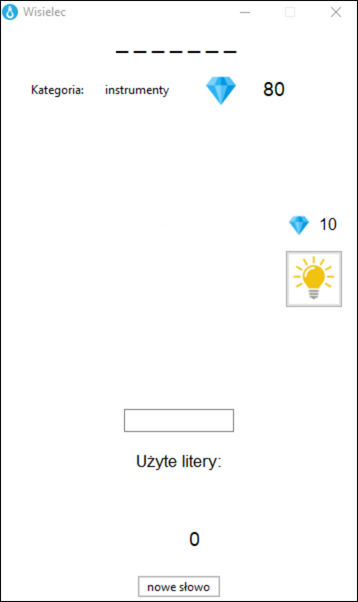
\includegraphics[width=\linewidth]{1}
		\caption{Początek rozgrywki}
		\label{fig:rozpoczecie_gry}
		\vspace{0.5cm} % Dodaj odstęp 0.5 cm
	\end{subfigure}
	\hspace{1cm} % Dodaj odstęp 1 cm
	\begin{subfigure}{0.4\textwidth}
		\begin{subfigure}{0.4\textheight}
			\centering
			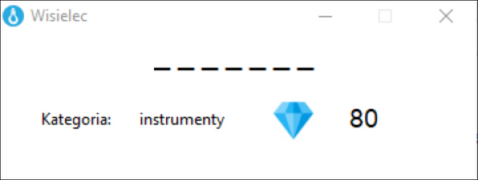
\includegraphics[width=0.8\linewidth]{2}
			\caption{Kategoria słowa i aktualna liczba punktów}
			\label{fig:kategoria_punkty}
			\vspace{2cm}
		\end{subfigure}
		\vspace{2cm} % Dodaj odstęp 0.5 cm
		\begin{subfigure}{0.4\textheight}
			\centering
			
\includegraphics[width=0.8\linewidth]{3}
			\caption{Użyte litery i liczba zwycięstw}
			\label{fig:uzyte_slowa_zywciestwa}
		\end{subfigure}
	\end{subfigure}
	\caption{Rozpoczęcie gry}
	\label{fig:Interface_menu}
\end{figure}

\subsection*{2. Zgadywanie liter}
\addcontentsline{toc}{subsection}{3.2 Zgadywanie liter}

Gracz wprowadza litery do pola tekstowego, próbując odgadnąć słowo. Jeżeli słowo zostało już wykorzystane (znajduje się w zbiorze \textit{"Użyte litery"}), pojawia się odpowiedni komunikat (rysunek~\ref{fig:litera_uzyta}). W przeciwnym przypadku następuje sprawdzenie, czy podana litera znajduje się w ukrytym słowie.

\vspace{0.5cm} % Dodaj odstęp 0.5 cm

\begin{figure}[h]
	\centering
	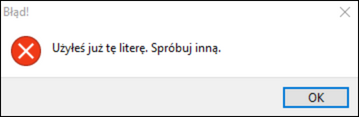
\includegraphics[width=0.6\linewidth]{uzyta_litera}
	\caption{Komunikat o błędzie ponownego wpisania tej samej litery}
	\label{fig:litera_uzyta}
\end{figure}

\subsubsection*{Poprawna odpowiedź}
\addcontentsline{toc}{subsubsection}{3.2.1 Poprawna odpowiedź}

Jeżeli litera występuje w słowie, wszystkie jej wystąpienia zostają odkryte na swoich odpowiednich pozycjach (rysunek~\ref{fig:poprawna_odpowiedz}), a gracz może kontynuować zgadywanie kolejnych liter. Dodatkowo, zgadnięta litera pojawia się wśród liter już użytych.

\subsubsection*{Niepoprawna odpowiedź}
\addcontentsline{toc}{subsubsection}{3.2.2 Niepoprawna odpowiedź}

Jeżeli litera nie występuje w słowie liczba dostępnych prób zostaje zmniejszona o jeden, co zwiększa trudność gry. Dodatkowo, rysowany jest kolejny element postaci wisielca (rysunek~\ref{fig:bledna_odpowiedz}), co stanowi wizualną reprezentację błędnej odpowiedzi. Ta dynamiczna zmiana wizualna motywuje gracza do większej ostrożności i trafności w kolejnych próbach. Ponadto, tak jak poprzednio, litera zostaje dopisana do zbioru użytych liter.

\vspace{0.5cm}

\begin{figure}[h]
	\centering
	\begin{subfigure}{0.4\textwidth}
		\centering
		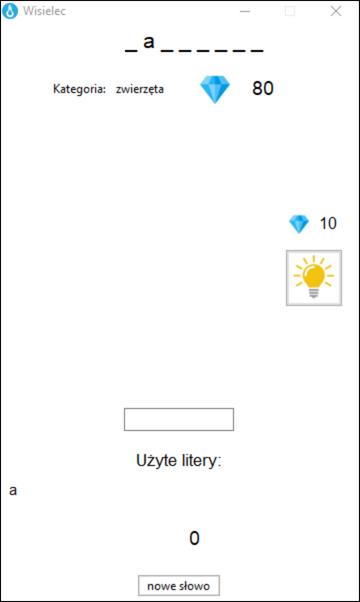
\includegraphics[width=\linewidth]{5}
		\caption{Poprawna odpowiedź}
		\label{fig:poprawna_odpowiedz}
	\end{subfigure}
	\hspace{1cm} % Dodaj odstęp 1 cm
	\begin{subfigure}{0.4\textwidth}
			\centering
			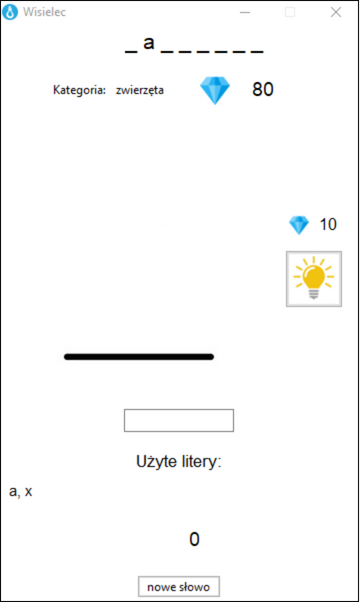
\includegraphics[width=\linewidth]{6}
			\caption{Błędna odpowiedź}
			\label{fig:bledna_odpowiedz}
		\end{subfigure}
	\caption{Sprawdzenie poprawności odpowiedzi}
	\label{fig:Poprawnosc_odpowiedzi}
\end{figure}

\newpage

\subsection*{3. Wyświetlenie podpowiedzi (opcjonalne)}
\addcontentsline{toc}{subsection}{3.3 Wyświetlenie podpowiedzi}

Jeżeli gracz ma $\geq10$ punktów, może skorzystać z podpowiedzi, co skutkuje zmniejszeniem aktualnego zasobu punktów o 10. Po jej użyciu jedna litera w zgadywanym słowie zostaje odsłonięta w każdym miejscu, w którym występuje w słowie (rysunek~\ref{fig:podpowiedz}) oraz zostaje dołączona do zbioru \textit{"Użyte litery"}. Podpowiedź może znacząco ułatwić proces odgadywania słowa, pomagając graczowi dokładniej określić jego zawartość. 
\vspace{0.25cm}
\\Jeżeli zaś gracz ma $0$ punktów, po naciśnięciu przycisku oznaczającego podpowiedź, wyświetla się odpowiedni komunikat (rysunek~\ref{fig:za_malo_diamentow}).
\vspace{0.25cm}
\\W przypadku, gdy słowo zostało już odgadnięte, a naciśnięto przycisk podpowiedzi wyświetli się komunikat o zakończonej grze (rysunek~\ref{fig:koniec_gry}).

\vspace{0.5cm}

\begin{figure}[h]
	\centering
	\begin{subfigure}{0.4\textwidth}
		\centering
		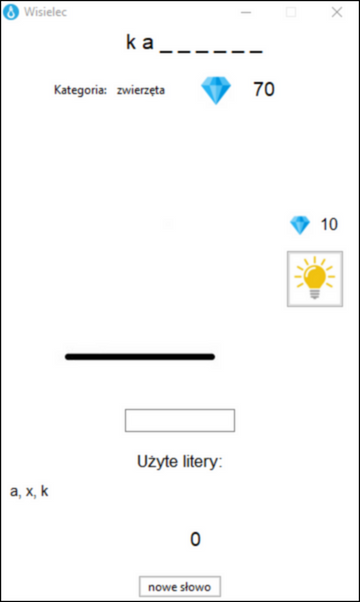
\includegraphics[width=\linewidth]{7}
		\caption{Podpowiedź}
		\label{fig:podpowiedz}
		\vspace{0.5cm} % Dodaj odstęp 0.5 cm
	\end{subfigure}
	\begin{subfigure}{0.4\textwidth}
		\begin{subfigure}{0.4\textheight}
			\centering
			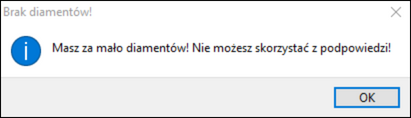
\includegraphics[width=0.8\linewidth]{brak_diamentow}
			\caption{Komunikat o zbyt małej liczbie punktów(diamentów)}
			\label{fig:za_malo_diamentow}
			\vspace{2cm}
		\end{subfigure}
		\vspace{2cm} % Dodaj odstęp 0.5 cm
		\begin{subfigure}{0.4\textheight}
			\centering
			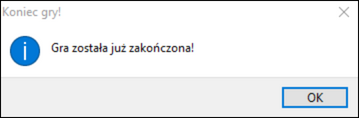
\includegraphics[width=0.8\linewidth]{koniec_gry}
			\caption{Komunikat o zakończeniu gry}
			\label{fig:koniec_gry}
		\end{subfigure}
	\end{subfigure}
	\caption{Działanie przycisku podpowiedzi}
	\label{fig:Podpowiedz}
\end{figure}

\subsection*{4. Zakończenie gry}
\addcontentsline{toc}{subsection}{3.4 Zgadywanie liter}

Gra kończy się, gdy gracz odgadnie całe słowo (zwycięstwo) lub popełni maksymalną liczbę błędów (porażka).

\subsubsection*{Zwycięstwo}
\addcontentsline{toc}{subsubsection}{3.4.1 Zwycięstwo}

Gdy gracz odgadnie wszystkie litery w tajnym słowie, gra kończy się zwycięstwem. W tym momencie gracz otrzymuje komunikat o sukcesie (rysunek~\ref{fig:zwyciestwo}), liczba punktów zwiększa się o 10 (rysunek~\ref{fig:zwyciestwo_punkty}), a następnie gra może być kontynuowana (przez użycie przycisku \textit{"nowa gra"}) lub zakończona.

\begin{figure}[h]
	\centering
	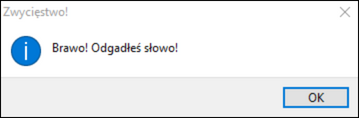
\includegraphics[width=0.5\linewidth]{zwyciestwo}
	\caption{Komunikat o zwycięstwie}
	\label{fig:zwyciestwo}
\end{figure}
\begin{figure}[h]
	\centering
	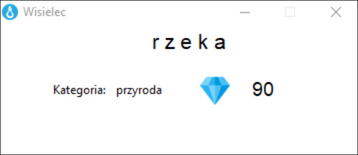
\includegraphics[width=0.5\linewidth]{8}
	\caption{Zwiększenie liczby punktów (diamentów) o 10}
	\label{fig:zwyciestwo_punkty}
\end{figure}

\FloatBarrier

Jednocześnie, zwiększana jest również liczba odniesionych zwycięstw (rysunek~\ref{fig:zwyciestwa_plus}). Jeżeli gracz wygrał po raz 5, to przy liczbie zwycięstw pojawia się puchar brązowy (najniższy poziom w grze) (rysunek~\ref{fig:puchar5}). Po 10 zwycięstwach puchar zmienia się na srebrny, a po 15 na złoty. Puchary odpowiadające kolejnym osiąganym poziomom w grze są przedstawione na rysunku~\ref{fig:puchary}.

\begin{figure}[H]
	\begin{subfigure}{0.5\textwidth}
		\centering
		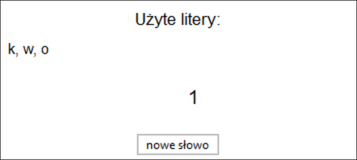
\includegraphics[width=1\linewidth]{9}
		\caption{Zwiększenie liczby zwycięstw}
		\label{fig:zwyciestwa_plus}
	\end{subfigure}
	\hspace{0.5cm}
	\begin{subfigure}{0.5\textwidth}
		\centering
		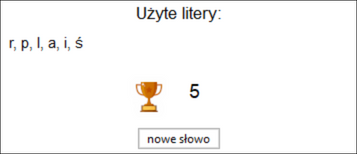
\includegraphics[width=1\linewidth]{10}
		\caption{Wyświetlenie pucharu brązowego przy 5-tej wygranej}
		\label{fig:puchar5}
	\end{subfigure}
	\caption{Zwiększanie liczby zwycięstw i wyświetlanie pucharów}
\end{figure}
\begin{figure}[H]
	\centering
	\begin{subfigure}{0.3\textwidth}
		\centering
		
\includegraphics[width=0.25\linewidth]{puchar_1}
		\caption{Puchar brązowy}
		\label{fig:puchar_brazawy}
	\end{subfigure}
	\begin{subfigure}{0.3\textwidth}
		\centering
		
\includegraphics[width=0.25\linewidth]{puchar_2}
		\caption{Puchar srebrny}
		\label{fig:puchar_srebrny}
	\end{subfigure}
	\begin{subfigure}{0.3\textwidth}
		\centering
		
\includegraphics[width=0.25\linewidth]{puchar_3}
		\caption{Puchar złoty}
		\label{fig:puchar_zloty}
	\end{subfigure}
	\caption{Puchary odpowiadające kolejnym osiąganym poziomom w grze}
	\label{fig:puchary}
\end{figure}

\FloatBarrier
\subsection*{Porażka}
\addcontentsline{toc}{subsubsection}{3.4.2 Porażka}
\FloatBarrier
Gdy gracz przegra w grze, czyli popełni maksymalną dopuszczalną liczbę błędów (10), następuje zakończenie gry. W tym momencie pojawi się komunikat informujący gracza o przegranej (rysunek~\ref{fig:porazka}). Gracz nie otrzymuje punktów za przegraną rundę. Gra może być kontynuowana (przycisk \textit{"nowa gra"}) lub zakończona.

\FloatBarrier
\begin{figure}[H]
	\centering
	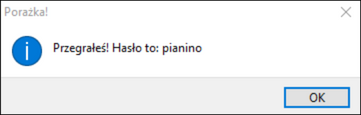
\includegraphics[width=0.5\linewidth]{porazka}
	\caption{Komunikat o porażce}
	\label{fig:porazka}
\end{figure}

\vspace{0.1cm}
Zarówno w przypadku zwycięstwa, jak i porażki, gdy po wyświetleniu komunikatu o wyniku gry użytkownik spróbuje wpisać kolejną literę, wyświetli się komunikat o końcu gry (rysunek~\ref{fig:koniec}).

\FloatBarrier
\begin{figure}[H]
	\centering
	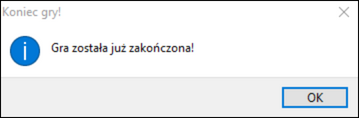
\includegraphics[width=0.5\linewidth]{koniec_gry}
	\caption{Komunikat o zakończeniu gry}
	\label{fig:koniec}
\end{figure}

\subsection*{5. Rozpoczęcie nowej rundy}
\addcontentsline{toc}{subsection}{3.5 Porażka}

Po zakończeniu aktualnej rundy, gracz może nacisnąć przycisk \textit{"nowe słowo"}, aby rozpocząć kolejną rundę i odgadnąć nowe słowo. Liczba zwycięstw i punkty (diamenty) zostaną zapisane do kolejnej rundy (rysunek~\ref{fig:nowa_gra}).

\FloatBarrier
\begin{figure}[H]
	\centering
	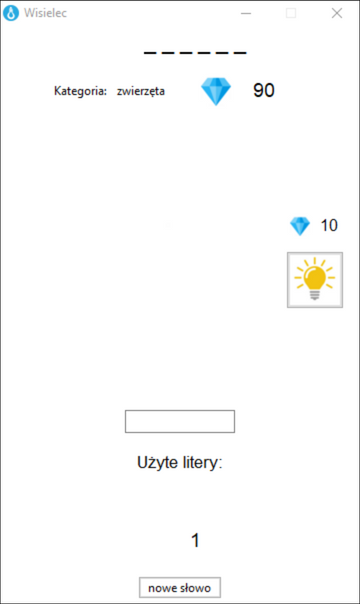
\includegraphics[width=0.45\linewidth]{11}
	\caption{Nowa gra}
	\label{fig:nowa_gra}
\end{figure}

\newpage
\section *{Struktura Kodu}
\addcontentsline{toc}{section}{3. Struktura kodu}
Kod źródłowy składa się z jednego pliku nagłówkowego i jednego pliku  \texttt{cpp}. 

\subsection*{wisielecMain.h}
\addcontentsline{toc}{subsection}{3.1 Plik wisielecMain.h}

Plik nagłówkowy w języku C++ definiuje główną klasę dialogową (wwisielecDialog) dla aplikacji opartej na bibliotece wxWidgets. Oto kilka kluczowych elementów pliku:
	
\begin{itemize}
	
	\item \textbf{Dołączenie bibliotek:} Plik dołącza standardowe nagłówki biblioteki C++ (<vector> i <fstream>) oraz definiuje makro, które przekształca tekst z kodowania UTF-8 na obiekt wxString w języku C++.
	
		\begin{lstlisting}
			//...
			#include <vector>
			#include <fstream>
			#include <wx/msgdlg.h>
			//...
			#undef _
			#define _(s) wxString::FromUTF8(s)
			//...
		\end{lstlisting}
		
	\item \textbf{Deklaracja klasy:} Jest to deklaracja klasy wwisielecDialog, dziedziczącej po klasie wxDialog, która reprezentuje główne okno dialogowe aplikacji.
		
		\begin{lstlisting}
			class wisielecDialog: public wxDialog
			{
				// ... (treść klasy)
			};
		\end{lstlisting}
		
		\item \textbf{Metody publiczne:} Na początku deklarowany jest konstuktor i destruktor klasy wisielecDialog. Następnie dodaliśmy własne funckje umożliwiające lepszą przejżystość kodu i zmniejszenie redundancji.
		
		\begin{lstlisting}
			//...
			public:
			wisielecDialog(wxWindow* parent,wxWindowID id = -1);
			virtual ~wisielecDialog();
			void InitializeGame();
			void UpdateCupImage();
			void LoadWordsFromFile(const wxString& fileName);
			//...
		\end{lstlisting}
\begin{itemize}
		\item \textit{\textbf{void InitializeGame();}} Inicjalizuje nową grę w wisielca, losując słowo i kategorię, resetując stan gry i aktualizując interfejs.
			
		\item \textit{\textbf{void UpdateCupImage();}} Aktualizuje obraz pucharu w zależności od liczby wygranych. 
			
		\item \textit{\textbf{void LoadWordsFromFile(const wxString $\&{}$ fileName);}} Wczytuje słowa i kategorie z pliku tekstowego do dwóch list (wordsList i categoriesList). Każdy wiersz w pliku powinien zawierać parę kategoria-słowo, oddzieloną spacją. 
			
			
\end{itemize}

\newpage
		
	\item \textbf{Pola prywatne:} Stworzyliśmy kilka zmiennych, używanych przez naszą gre.
		
		\begin{lstlisting}
			//...
			private:
			wxString secretWord;
			wxString guessedWord;
			wxString usedLetters;
			wxString category;
			wxString remainingLetters;
			bool gameFinished;
			int incorrectGuesses;
			int currentHangmanImage = 0;
			int points = 80;
			int wins=0;
			std::vector<wxString> wordsList;
			std::vector<wxString> categoriesList;
			//...
		\end{lstlisting}
		
\begin{itemize}
		\item \textit{\textbf{wxString secretWord;}} Przechowuje ukryte słowo, które gracz musi odgadnąć.
			
		\item \textbf{\textit{wxString guessedWord;}} Zawiera aktualne odgadnięte litery z ukrytego słowa w formie tekstowej, gdzie nieodgadnięte litery są zastępowane znakiem podkreślenia.
			
		\item \textit{\textbf{wxString usedLetters;}} Zawiera litery, które gracz już użył podczas gry.
			
		\item \textit{\textbf{wxString category;}} Przechowuje kategorię, do której należy ukryte słowo.
			
		\item \textit{\textbf{wxString remainingLetters;}} Zawiera litery, które pozostały do odgadnięcia w ukrytym słowie.
			
		\item \textit{\textbf{bool gameFinished;}} Wartość logiczna informująca o stanie gry (czy gra została zakończona).
			
		\item \textit{\textbf{int incorrectGuesses;}} Liczba nieudanych prób odgadnięcia litery.
			
		\item \textit{\textbf{int currentHangmanImage=0;}}Numer aktualnego obrazu w grze w wisielca, domyślnie zadeklarowany jako 0.
			
		\item \textit{\textbf{int points = 80;}} Liczba punktów zdobytych w trakcie gry, domyślnie ustawione na 80.
			
		\item \textit{\textbf{int wins = 0;}} Liczba zwycięstw w grze, domyślnoie ustawiona na 0.
			
		\item \textit{\textbf{std::<wxString> wordsList;}}Wektor przechowujący słowa, które można odgadnąć w grze.
			
		\item \textit{\textbf{std::<wxString> categoriesList;}} Wektor przechowujący kategorie odpowiadające słowom w wordsList.
			
		\end{itemize}
		
	\end{itemize}
	
\newpage
	
\subsection*{wisielecMain.cpp}
\addcontentsline{toc}{subsection}{3.2. Plik wisielecMain.cpp}
	
Plik $wisielecMain.cpp$ zawiera implementację głównego okna aplikacji \textit{"Wisielec"}. Znajdują się w nim definicje funkcji obsługujących zdarzenia interakcji użytkownika. Dodatkowo, plik zawiera definicje funkcji pomocniczych oraz konstruktor i destruktor klasy $wisielecDialog$, które odpowiadają za inicjalizację interfejsu użytkownika. Oto jego podstawowe elementy:

	\begin{itemize}
		\item \textbf{Początek pliku:} Na początku dołączamy dyrektywy $\#$include używane do wczytania nagłówków z różnych bibliotek. Wśród nich znajdują się m.in. $wx/msgdlg.h$ dla obsługi okien dialogowych wiadomości w wxWidgets, "wisielecMain.h" dla lokalnego pliku nagłówkowego związanego z głównym oknem aplikacji "wisielec", $<sstream>$ dla operacji na strumieniach w C++ oraz $<wx/log.h>$ dla logowania w aplikacji wxWidgets.
		\begin{lstlisting}
	#include <wx/msgdlg.h>
	//...
	#include "wisielecMain.h"
	#include <sstream>
	#include <wx/log.h>
		\end{lstlisting}
		\item \textbf{Konstruktor klasy wisielecDialog:} Inicjuje elementy interfejsu użytkownika oraz przygotowuje stan gry do rozpoczęcia, ustawiając ikonę aplikacji oraz inicjując generator liczb pseudolosowych.
		\begin{lstlisting}
	wisielecDialog::wisielecDialog(wxWindow* parent,wxWindowID id)
	{
		//...
		SetIcon(wxICON(aaaa));
		this->FlexGridSizer1 = FlexGridSizer1;
		srand(time(0));
		InitializeGame();
	}
		\end{lstlisting}
		\begin{itemize}
			\item \textbf{\textit{SetIcon(wxICON(aaaa));}} Ustawia ikonę okna dialogowego.
			\item \textbf{\textit{this->FlexGridSizer1 = FlexGridSizer1;}} Przypisuje wskaźnik do utworzonej siatki rozmieszczenia (\textit{FlexGridSizer1}) do odpowiedniego pola (\textit{FlexGridSizer1}) w obiekcie $wisielecDialog$.
			\item \textbf{\textit{srand(time(0));}} Inicjalizuje generator liczb pseudolosowych srand przy użyciu aktualnego czasu jako ziarna.
			\item \textbf{\textit{InitializeGame();}} Wywołuje metodę inicjalizującą grę.
			
		\end{itemize}
		\item \textbf{OnButton1Click:} Obsługuje zdarzenie przetworzenia nowo wpisanej litery w polu tekstowym. Oto jego kolejne składowe:
		\begin{itemize}
			\item Pobiera wartość wprowadzoną przez użytkownika do pola tekstowego $TextCtrl1$ i przypisuje ją do zmiennej $input$ typu $wxString$. Ta wartość to litera wprowadzona przez użytkownika w celu odgadnięcia słowa w grze.
			\begin{lstlisting}
{
	wxString input = TextCtrl1->GetValue();
	//...
			\end{lstlisting}
			\newpage
			\item Ten fragment służy do obsługi wprowadzania liter przez użytkownika w polu tekstowym ($TextCtrl1$). Po pobraniu wartości wprowadzonej przez użytkownika do zmiennej $input$, kod sprawdza, czy gra nie została zakończona ($!gameFinished$) oraz czy wprowadzona wartość jest pojedynczą literą alfabetu. Jeśli tak, to sprawdzane jest, czy wprowadzona litera nie została wcześniej użyta. Jeśli nie, jest ona dodawana do listy użytych liter ($usedLetters$).
			\begin{lstlisting}
	//...
	if(!gameFinished)
	{
		if (input.length() == 1 && wxIsalpha(input[0]))
		{
			auto guessedLetter = input[0];
			
			if (usedLetters.find(guessedLetter) == wxString::npos)
			{
				if(usedLetters.length()==0)
				{
					usedLetters = wxString(guessedLetter);
				}
				else
				{
					usedLetters +=   ", " + wxString(guessedLetter);
				}
	//...
			\end{lstlisting}
			\item Sprawdzenie, czy wprowadzona litera jest częścią tajnego słowa ($secretWord$). Jeśli tak, aktualizowana jest wyświetlana odgadnięta część słowa ($guessedWord$), w której każda litera jest reprezentowana przez znak podkreślenia. Jeśli litera występuje w tajnym słowie, jej odpowiednie miejsce w $guessedWord$ jest zastępowane wprowadzoną literą, a wartość zmiennej $correctGuess$ jest ustawiana na $true$.
			
			\begin{lstlisting}
	//...
				bool correctGuess = false;
				guessedWord = StaticText1->GetLabel();
				for (size_t i = 0; i < secretWord.length(); ++i)
				{
					if (secretWord[i] == guessedLetter)
					{
						guessedWord[i * 2] = guessedLetter;
						correctGuess = true;
					}
				}
			//...
			\end{lstlisting}
			\item Jeśli wprowadzona litera została odgadnięta poprawnie (czyli występuje w tajnym słowie), aktualizowane jest wyświetlane odgadnięte słowo ($guessedWord$) na etykiecie statycznej ($StaticText1$). Jeśli nie, nic nie jest aktualizowane.
			\begin{lstlisting}
				//...
				if (correctGuess) {
					StaticText1->SetLabel(guessedWord);
				}
				//...
			\end{lstlisting}
	\newpage
			\item Jeśli wszystkie litery w tajnym słowie zostały odgadnięte (nie ma już znaków podkreślenia $"\_"$ w $guessedWord$), wyświetlane jest okno dialogowe gratulujące zwycięstwa. Dodatkowo, przycisk \textit{"nowe słowo"} jest aktywowany, a punkty oraz liczba wygranych są zaktualizowane, a następnie wyczyszczony jest $TextCtrl1$, aby użytkownik mógł zacząć odgadywanie nowego słowa.
			\begin{lstlisting}
				//...
				if (guessedWord.find('_') == wxString::npos)
				{
					wxMessageBox(_("Brawo! Odgadłeś słowo!"), _("Zwycięstwo!"), wxOK | wxICON_INFORMATION);
					TextCtrl1->Clear();
					gameFinished=true;
					wins+=1;
					UpdateCupImage();
					StaticText7->SetLabelText(wxString::Format(_("%d"), wins));
					points+=10;
					StaticText6->SetLabel(wxString::Format(_("%d"), points));
					return;
				}
				//...
			\end{lstlisting}
			\item Linia $TextCtrl1->Clear();$ czyści zawartość kontrolki $TextCtrl1$, która służy do wprowadzania liter przez użytkownika podczas odgadywania słowa. Po udanym odgadnięciu słowa, ta linia usuwa wprowadzoną literę, aby użytkownik mógł zacząć wprowadzać nową literę bez konieczności ręcznego usuwania poprzedniej.
			\begin{lstlisting}
				//...
				TextCtrl1->Clear();
				//...
			\end{lstlisting}
			\item Ten fragment kodu obsługuje przypadki, gdy wprowadzona litera nie znajduje się w tajnym słowie. Gdy wprowadzona litera nie jest częścią słowa, zwiększa licznik niepoprawnych prób $incorrectGuesses$, co oznacza, że wisielec jest rysowany stopniowo. Następnie aktualizowany jest obraz wisielca poprzez zmianę mapy bitowej na kolejną fazę wisielca. Jeśli liczba niepoprawnych prób osiągnie 10, użytkownik otrzymuje komunikat informujący, że przegrał, a jednocześnie wyświetlone jest tajne słowo.
			\begin{lstlisting}
				//...
				if (!correctGuess)
				{
					incorrectGuesses++;
					
					currentHangmanImage++;
					
					wxString imageName = wxString::Format("wisielec%d.jpg", currentHangmanImage);
					wxBitmap hangmanBitmap(imageName, wxBITMAP_TYPE_JPEG);
					
					if (hangmanBitmap.IsOk())
					{
						StaticBitmap1->SetBitmap(hangmanBitmap);
					}
					
					if (incorrectGuesses == 10)
					{
						wxMessageBox(_("Przegrałeś! Hasło to: ") + secretWord, _("Porażka!"), wxOK | wxICON_INFORMATION);
					}
				}			
				//...
			\end{lstlisting}
			\item Aktualizowanie etykiety $StaticText3$, aby wyświetlić litery, które zostały już użyte przez gracza. Zawiera to zarówno poprawne, jak i niepoprawne próby zgadywania liter.
			\begin{lstlisting}
				//...
				StaticText3->SetLabel(usedLetters);
				}
				//...
			\end{lstlisting}
			\item Wyświetlenie komunikatu błędu, jeśli gracz próbuje użyć litery, którą już wcześniej użył. Następnie czyszczone jest pole tekstowe $TextCtrl1$, aby umożliwić graczowi wprowadzenie nowej litery.
			\begin{lstlisting}
				//...
				else
				{
					wxMessageBox(_("Użyłeś już tę literę. Spróbuj inną."), _("Błąd!"), wxOK | wxICON_ERROR);
					TextCtrl1->Clear();
				}
				}
			}
			//...
			\end{lstlisting}
			\item Sprawdzenie, czy gra została już zakończona ($gameFinished$). Jeśli tak, wyświetlany jest komunikat informacyjny o zakończeniu gry. Następnie funkcja kończy swoje działanie.
			\begin{lstlisting}
			//...
			else
			{
				wxMessageBox(_("Gra została już zakończona!"), _("Koniec gry!"), wxOK | wxICON_INFORMATION);
				return;
			}
		}
			\end{lstlisting}
		\end{itemize}
		\item \textbf{InitializeGame:} Funkcja rozpoczyna nową grę, losując słowo i kategorię, resetując stan gry i przywracając ustawione w niej domyślne ustawienia. Oto opis jej kolejnych elementów:
		\begin{itemize}
			\item Wczytywanie słów i kategorii z pliku \textit{"slowa.txt"}, a następnie losowanie słowa i odpowiadającej mu kategorii.
			\begin{lstlisting}
	//...
	{
		LoadWordsFromFile("slowa.txt");
		
		size_t wordIndex = rand() % wordsList.size();
		secretWord = wordsList[wordIndex];
		category = categoriesList[wordIndex];
		//...
			\end{lstlisting}
			\item Resetowanie gry: ustawianie pustej zmiennej $guessedWord$ na ciąg znaków $"\_"$ o długości równej tajnemu słowu, czyszczenie użytych liter, resetowanie liczby błędnych prób, ustawianie zmiennej $gameFinished$ na fałsz (gra nie jest zakończona).
			\begin{lstlisting}
		//...
		guessedWord="";
		for (int i=0; i< secretWord.length();i++)
		guessedWord += "_ ";
		usedLetters.clear();
		incorrectGuesses = 0;
		gameFinished = false;
		//...
			\end{lstlisting}
			\item Aktualizacja etykiety tekstowej w interfejsie użytkownika: ustawienie wartości dla odgadniętego słowa ($guessedWord$), użytych liter ($usedLetters$), kategorii ($category$), liczby zwycięstw ($wins$), oraz punktów ($points$).
			\begin{lstlisting}
		//...
		StaticText1->SetLabel(guessedWord);
		StaticText3->SetLabel(usedLetters);
		StaticText5->SetLabel(category);
		StaticText7->SetLabelText(wxString::Format(_("%d"), wins));
		StaticText6->SetLabel(wxString::Format(_("%d"), points));
		//...
			\end{lstlisting}
			\item Ustawienie obrazu wisielca na początkowy, czyszczenie pola tekstowego oraz wczytanie obrazu wisielca o nazwie \textit{"wisielec0.jpg"}.
			\begin{lstlisting}
		//...
		currentHangmanImage = 0;
		TextCtrl1->Clear();
		wxString imageName = wxString::Format("wisielec0.jpg");
		wxBitmap hangmanBitmap(imageName, wxBITMAP_TYPE_JPEG);
		//...
			\end{lstlisting}
			\item Ten fragment sprawdza, czy obraz wisielca został poprawnie wczytany, a następnie ustawia ten obraz w kontrolce statycznej ($StaticBitmap1$).
			\begin{lstlisting}
		//...
		if (hangmanBitmap.IsOk())
		{
			StaticBitmap1->SetBitmap(hangmanBitmap);
		}
		
	}
			\end{lstlisting}
		\end{itemize}
		\item \textbf{OnButton2Click:} Funkcja obsługuje kliknięcie przycisku \textit{"nowe słowo"} w interfejsie. Oto kolejne kroki tej funkcji:
		\begin{itemize}
			\item Wywołanie metody $InitializeGame()$, która przygotowuje nową grę, losując nowe słowo, resetując stan gry i przywracając domyślny obraz wisielca. 
			\begin{lstlisting}
	{
		InitializeGame();			
	}
			\end{lstlisting}
		\end{itemize}
			\item \textbf{LoadWordsFromFile:} Funkcja obsługuje kliknięcie przycisku \textit{"nowe słowo"} w interfejsie. Oto kolejne kroki tej funkcji:
			\begin{itemize}
			\item Funkcja otwiera plik tekstowy $fileName$ i wczytuje z niego listę słów do odgadnięcia wraz z ich kategoriami. Następnie każde słowo i jego kategoria są dodawane do odpowiednich list $wordsList$ i $categoriesList$. Jeśli format wiersza w pliku jest nieprawidłowy, generowany jest odpowiedni komunikat logu. W przypadku błędu otwarcia pliku, wyświetlany jest komunikat błędu, informujący użytkownika o problemie z otwarciem pliku.
			\begin{lstlisting}
	{
		std::ifstream file(fileName.ToStdString());
		if (file.is_open()) {
			std::string line;
			while (std::getline(file, line)) {
				std::istringstream iss(line);
				std::string category, word;
				
				if (iss >> category >> std::ws && std::getline(iss, word)) {
					wordsList.push_back(wxString::FromUTF8(word.c_str()));
					categoriesList.push_back(wxString::FromUTF8(category.c_str()));
				} else {
					wxLogMessage(_("Nieprawidłowy format wiersza: %s"), wxString::FromUTF8(line.c_str()));
				}
			}
			file.close();
		} else {
			wxLogError(_("Nie udało się otworzyć pliku: %s"), wxString::FromUTF8(fileName.c_str()));
			wxMessageBox(wxString::FromUTF8(_("Nie udało się otworzyć pliku ")) + fileName, wxString::FromUTF8(_("Błąd!")), wxOK | wxICON_ERROR);
		}
	}
			\end{lstlisting}
		\end{itemize}
		\item \textbf{OnBitmapButton1Click:} Metoda obsługuje kliknięcie przycisku podpowiedzi.
		\begin{itemize}
			\item Jeśli gra nie została zakończona i liczba błędnych prób jest mniejsza niż 10, funkcja sprawdza, czy sekretny wyraz jest pusty. Jeśli tak, wyświetla komunikat o błędzie informujący o braku słowa do odgadnięcia.
			\begin{lstlisting}
	{
		if(!gameFinished && incorrectGuesses<10)
		{
			if (secretWord.empty()) {
				wxMessageBox(_("Brak słowa do odgadnięcia!"), _("Błąd!"), wxOK | wxICON_ERROR);
				return;
			}
			//...
			\end{lstlisting}
	\newpage
			\item Jeśli gracz ma co najmniej 10 punktów, funkcja sprawdza, które litery w sekretnym wyrazie jeszcze nie zostały odgadnięte. Następnie losuje jedną z tych liter jako podpowiedź dla gracza.
			\begin{lstlisting}
			//...
			if (points >= 10)
			{
				wxString remainingLetters;
				for (size_t i = 0; i < secretWord.length(); ++i)
				{
					if (guessedWord[i * 2] == '_') {
						remainingLetters += secretWord[i];
					}
				}
				
				if (!remainingLetters.empty()) {
					points -= 10;
					StaticText6->SetLabel(wxString::Format(_("%d"), points));
					
					size_t randomIndex = rand() % remainingLetters.length();
					char randomLetter = remainingLetters[randomIndex];
					//...
			\end{lstlisting}
			\item Jeśli wylosowana litera nie została jeszcze użyta, dodaje ją do użytych liter. Następnie aktualizuje wyświetlane słowo, zastępując podkreślenia odgadniętymi literami.
			\begin{lstlisting}
					//...
					if (!usedLetters.empty()) {
						usedLetters += ", ";
					}
					usedLetters += wxString(randomLetter);
					StaticText3->SetLabel(usedLetters);
					
					for (size_t i = 0; i < secretWord.length(); ++i) {
						if (secretWord[i] == randomLetter) {
							guessedWord[i * 2] = randomLetter;
						}
					}
					
					StaticText1->SetLabel(guessedWord);
					//...
			\end{lstlisting}
			\item Jeśli odgadnięto wszystkie litery w słowie, wyświetla się wiadomość o zwycięstwie, aktualizując wynik gracza i obrazek pucharu oraz dodając punkty. W przeciwnym razie, jeśli liczba błędnych prób osiągnie 10, wyświetla się wiadomość o przegranej.
			\begin{lstlisting}
				//...
				if (guessedWord.find('_') == wxString::npos) {
					wxMessageBox(_("Brawo! Odgadłeś słowo!"), _("Zwycięstwo!"), wxOK | wxICON_INFORMATION);
					TextCtrl1->Clear();
					gameFinished=true;
					wins += 1;
					UpdateCupImage();
					StaticText7->SetLabelText(wxString::Format(_("%d"), wins));
					points += 10;
					StaticText6->SetLabel(wxString::Format(_("%d"), points));
					return;
				}
				else if (incorrectGuesses == 10)
				{
					wxMessageBox(_("Przegrałeś! Hasło to: ") + secretWord, _("Porażka!"), wxOK | wxICON_INFORMATION);
					TextCtrl1->Clear();
					gameFinished = true;
				}
				//...
			\end{lstlisting}
			\item Jeśli wszystkie litery w słowie zostały już odgadnięte, wyświetla się komunikat o braku dostępnych podpowiedzi.
			\begin{lstlisting}
			//...
			} else
			{
			wxMessageBox(_("Wszystkie litery zostały już odgadnięte!"), _("Brak podpowiedzi"), wxOK | wxICON_INFORMATION);
			}
			//...
			\end{lstlisting}
			\item Jeśli liczba punktów gracza jest mniejsza niż 10, wyświetla się komunikat informujący go o braku wystarczającej liczby punktów do skorzystania z podpowiedzi.
			\begin{lstlisting}
		//...
		} else
		{
		wxMessageBox(_("Masz za mało diamentów! Nie możesz skorzystać z podpowiedzi!"), _("Brak diamentów!"), wxOK | wxICON_INFORMATION);
		}
		//...
			\end{lstlisting}
			\item Jeśli gra została już zakończona, wyświetla się komunikat informujący gracza o końcu gry.
			\begin{lstlisting}
	//...
		}
	else
	{
		wxMessageBox(_("Gra została już zakończona!"), _("Koniec gry!"), wxOK | wxICON_INFORMATION);
		return;
	}
}
			\end{lstlisting}
		\end{itemize}
	\newpage
		\item \textbf{UpdateCupImage:} Metoda aktualizuje obrazek pucharu na podstawie liczby wygranych gracza.
		\vspace{0.25cm}
\\Funkcja aktualizuje obrazek pucharu na podstawie liczby wygranych. Jeśli liczba wygranych wynosi od 5 do 9, ustawia obrazek pucharu pierwszego poziomu. Jeśli liczba wygranych wynosi od 10 do 14, ustawia obrazek pucharu drugiego poziomu. Jeśli liczba wygranych wynosi 15 lub więcej, ustawia obrazek pucharu trzeciego poziomu. Na koniec odświeża obrazek pucharu.
\vspace{0.2cm}
			\begin{lstlisting}
{
	if (wins >= 5 && wins < 10)
	{
		StaticBitmap3->SetBitmap(wxBitmap(wxImage(("puchar_1.png"))));
	}
	else if (wins >= 10 && wins < 15)
	{
		StaticBitmap3->SetBitmap(wxBitmap(wxImage(_T("puchar_2.png"))));
	}
	else if (wins >= 15)
	{
		StaticBitmap3->SetBitmap(wxBitmap(wxImage(_T("puchar_3.png"))));
	}
	
	StaticBitmap3->Refresh();
}
			\end{lstlisting}
\end{itemize}
	
	\newpage

	\section*{Podział pracy}
	\addcontentsline{toc}{section}{4. Podział pracy}
	
	\begin{itemize}
		\item \textbf{Przygotowanie wyglądu okna dialogowego:}
		\subitem Bartosz Oleszek 60\%
		\subitem Katarzyna Zyśko 20\%
		\subitem Zuzanna Winiarska 20\%
		
		\item \textbf{Napisanie funkcji OnButton1Click:}
		\subitem Bartosz Oleszek 100\%
		\subitem Katarzyna Zyśko 0\%
		\subitem Zuzanna Winiarska 0\%
		
		\item \textbf{Napisanie funkcji InitializeGame:}
		\subitem Bartosz Oleszek 0\%
		\subitem Katarzyna Zyśko 0\%
		\subitem Zuzanna Winiarska 100\%
		
		\item \textbf{Napisanie funkcji OnButton2Click:}
		\subitem Bartosz Oleszek 0\%
		\subitem Katarzyna Zyśko 0\%
		\subitem Zuzanna Winiarska 100\%
		
		\item \textbf{Napisanie funkcji LoadWordsFromFile:}
		\subitem Bartosz Oleszek 0\%
		\subitem Katarzyna Zyśko 0\%
		\subitem Zuzanna Winiarska 100\%
		
		\item \textbf{Napisanie funkcji OnBitmapButton1Click:}
		\subitem Bartosz Oleszek 40\%
		\subitem Katarzyna Zyśko 0\%
		\subitem Zuzanna Winiarska 60\%
		
		\item \textbf{Napisanie funkcji UpdateCupImage:}
		\subitem Bartosz Oleszek 20\%
		\subitem Katarzyna Zyśko 20\%
		\subitem Zuzanna Winiarska 60\%
		
		\item \textbf{Przygotowanie dokumentacji:}
		\subitem Bartosz Oleszek 30\%
		\subitem Katarzyna Zyśko 40\%
		\subitem Zuzanna Winiarska 30\%
		
		\item \textbf{Ogólnie:}
		\subitem Bartosz Oleszek 30\%
		\subitem Katarzyna Zyśko 25\%
		\subitem Zuzanna Winiarska 35\%
	\end{itemize}
	
	\newpage
	
	\section*{Instrukcja instalacji}
	\addcontentsline{toc}{section}{5. Instrukcja instalacji}
	
	Instalator gry powstał przy pomocy aplikacji Createinstall. 
	
	\newpage
	
	\section*{Podsumowanie}
	\addcontentsline{toc}{section}{6. Podsumowanie}

Gra \textit{"Wisielec"} wyróżnia się przyjemną oprawą graficzną oraz prostą, lecz angażującą mechaniką, co ułatwia szybkie zrozumienie zasad gry. Różnorodność losowanych słów do odgadnięcia, wraz z możliwością korzystania z podpowiedzi, dodaje głębi rozgrywce, zapewniając graczom różnorodne wyzwania. Dodatkowo, zdobywanie pucharów za osiągnięcie określonej liczby zwycięstw stymuluje do dalszej gry, dodając element rywalizacji i motywując do osiągania coraz lepszych wyników.
	
	\vspace{0.5cm}

\textit{"Wisielec"} nie tylko dostarcza rozrywki, ale także wspomaga rozwój umiejętności logicznego myślenia oraz szybkiego podejmowania decyzji w sposób przystępny i angażujący. Dzięki wbudowanym elementom edukacyjnym stanowi atrakcyjną propozycję dla graczy pragnących zarówno bawić się, jak i doskonalić swoje umiejętności.
\end{document}
